% Created by tikzDevice version 0.12.6 on 2024-11-19 16:55:44
% !TEX encoding = UTF-8 Unicode
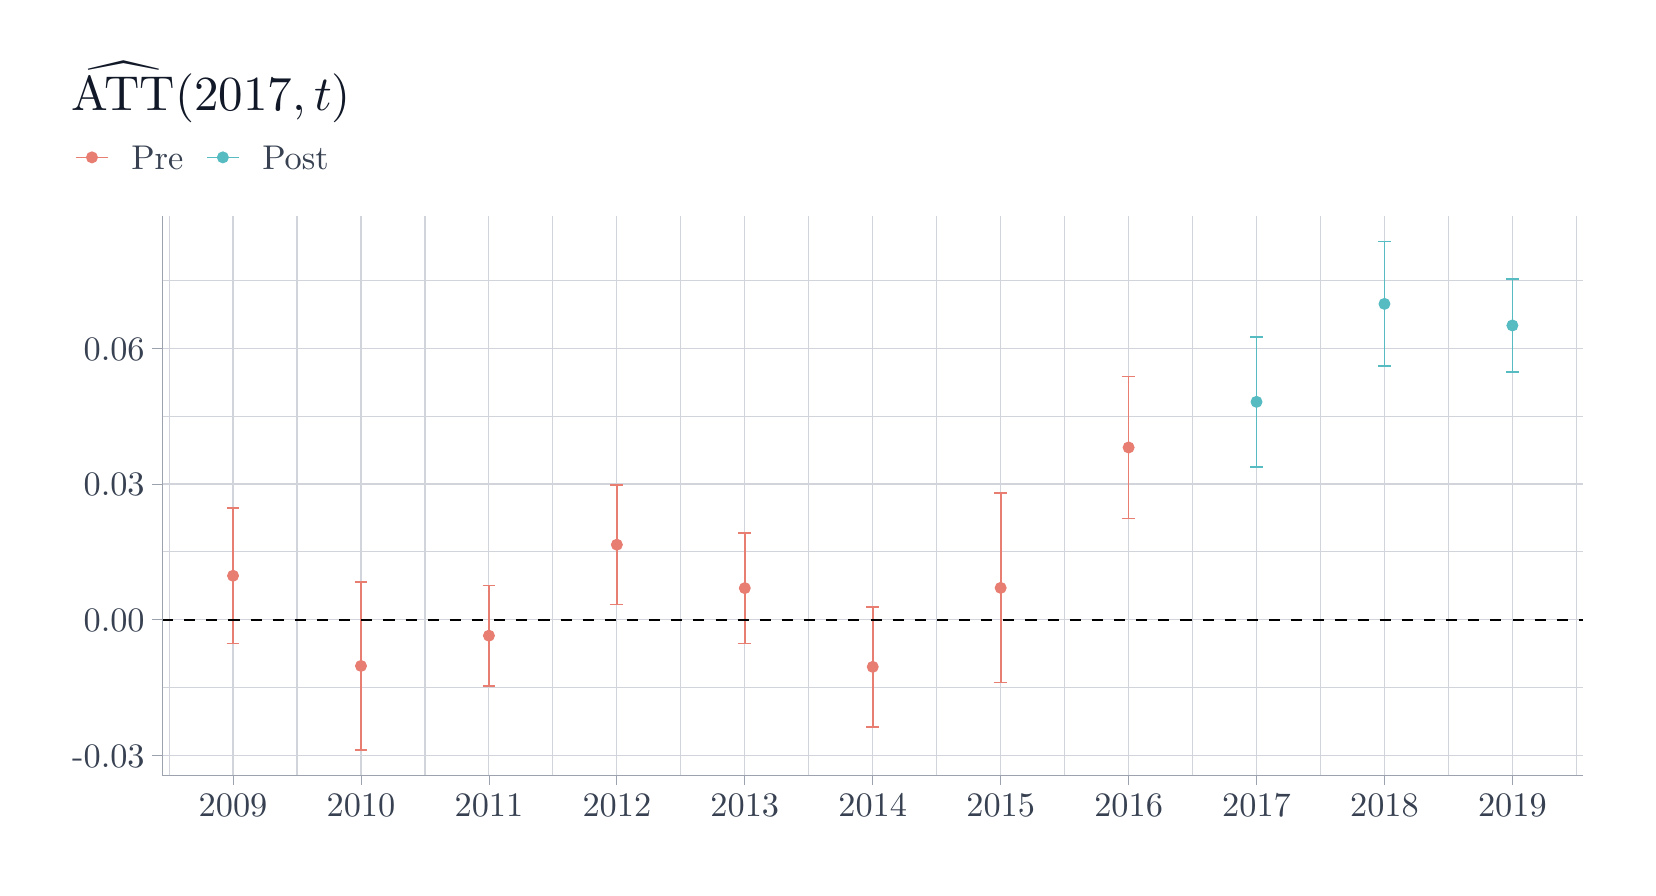
\begin{tikzpicture}[x=1pt,y=1pt]
\definecolor{fillColor}{RGB}{255,255,255}
\path[use as bounding box,fill=fillColor] (0,0) rectangle (578.16,303.53);
\begin{scope}
\path[clip] (  0.00,  0.00) rectangle (578.16,303.53);
\definecolor{drawColor}{RGB}{255,255,255}

\path[draw=drawColor,line width= 0.7pt,line join=round,line cap=round,fill=fillColor] (  0.00,  0.00) rectangle (578.16,303.53);
\end{scope}
\begin{scope}
\path[clip] ( 48.56, 33.29) rectangle (562.16,235.43);
\definecolor{drawColor}{RGB}{255,255,255}
\definecolor{fillColor}{RGB}{255,255,255}

\path[draw=drawColor,line width= 0.7pt,line join=round,line cap=round,fill=fillColor] ( 48.56, 33.29) rectangle (562.16,235.43);
\definecolor{drawColor}{RGB}{209,213,219}

\path[draw=drawColor,line width= 0.4pt,line join=round] ( 48.56, 65.02) --
	(562.16, 65.02);

\path[draw=drawColor,line width= 0.4pt,line join=round] ( 48.56,114.10) --
	(562.16,114.10);

\path[draw=drawColor,line width= 0.4pt,line join=round] ( 48.56,163.18) --
	(562.16,163.18);

\path[draw=drawColor,line width= 0.4pt,line join=round] ( 48.56,212.27) --
	(562.16,212.27);

\path[draw=drawColor,line width= 0.4pt,line join=round] ( 51.10, 33.29) --
	( 51.10,235.43);

\path[draw=drawColor,line width= 0.4pt,line join=round] ( 97.33, 33.29) --
	( 97.33,235.43);

\path[draw=drawColor,line width= 0.4pt,line join=round] (143.56, 33.29) --
	(143.56,235.43);

\path[draw=drawColor,line width= 0.4pt,line join=round] (189.79, 33.29) --
	(189.79,235.43);

\path[draw=drawColor,line width= 0.4pt,line join=round] (236.01, 33.29) --
	(236.01,235.43);

\path[draw=drawColor,line width= 0.4pt,line join=round] (282.24, 33.29) --
	(282.24,235.43);

\path[draw=drawColor,line width= 0.4pt,line join=round] (328.47, 33.29) --
	(328.47,235.43);

\path[draw=drawColor,line width= 0.4pt,line join=round] (374.70, 33.29) --
	(374.70,235.43);

\path[draw=drawColor,line width= 0.4pt,line join=round] (420.93, 33.29) --
	(420.93,235.43);

\path[draw=drawColor,line width= 0.4pt,line join=round] (467.16, 33.29) --
	(467.16,235.43);

\path[draw=drawColor,line width= 0.4pt,line join=round] (513.39, 33.29) --
	(513.39,235.43);

\path[draw=drawColor,line width= 0.4pt,line join=round] (559.62, 33.29) --
	(559.62,235.43);

\path[draw=drawColor,line width= 0.4pt,line join=round] ( 48.56, 40.48) --
	(562.16, 40.48);

\path[draw=drawColor,line width= 0.4pt,line join=round] ( 48.56, 89.56) --
	(562.16, 89.56);

\path[draw=drawColor,line width= 0.4pt,line join=round] ( 48.56,138.64) --
	(562.16,138.64);

\path[draw=drawColor,line width= 0.4pt,line join=round] ( 48.56,187.72) --
	(562.16,187.72);

\path[draw=drawColor,line width= 0.4pt,line join=round] ( 74.21, 33.29) --
	( 74.21,235.43);

\path[draw=drawColor,line width= 0.4pt,line join=round] (120.44, 33.29) --
	(120.44,235.43);

\path[draw=drawColor,line width= 0.4pt,line join=round] (166.67, 33.29) --
	(166.67,235.43);

\path[draw=drawColor,line width= 0.4pt,line join=round] (212.90, 33.29) --
	(212.90,235.43);

\path[draw=drawColor,line width= 0.4pt,line join=round] (259.13, 33.29) --
	(259.13,235.43);

\path[draw=drawColor,line width= 0.4pt,line join=round] (305.36, 33.29) --
	(305.36,235.43);

\path[draw=drawColor,line width= 0.4pt,line join=round] (351.59, 33.29) --
	(351.59,235.43);

\path[draw=drawColor,line width= 0.4pt,line join=round] (397.82, 33.29) --
	(397.82,235.43);

\path[draw=drawColor,line width= 0.4pt,line join=round] (444.04, 33.29) --
	(444.04,235.43);

\path[draw=drawColor,line width= 0.4pt,line join=round] (490.27, 33.29) --
	(490.27,235.43);

\path[draw=drawColor,line width= 0.4pt,line join=round] (536.50, 33.29) --
	(536.50,235.43);
\definecolor{drawColor}{RGB}{232,125,114}
\definecolor{fillColor}{RGB}{232,125,114}

\path[draw=drawColor,line width= 0.4pt,line join=round,line cap=round,fill=fillColor] ( 74.21,105.48) circle (  1.96);

\path[draw=drawColor,line width= 0.4pt,line join=round,line cap=round,fill=fillColor] (120.44, 72.89) circle (  1.96);

\path[draw=drawColor,line width= 0.4pt,line join=round,line cap=round,fill=fillColor] (166.67, 83.83) circle (  1.96);

\path[draw=drawColor,line width= 0.4pt,line join=round,line cap=round,fill=fillColor] (212.90,116.70) circle (  1.96);

\path[draw=drawColor,line width= 0.4pt,line join=round,line cap=round,fill=fillColor] (259.13,101.01) circle (  1.96);

\path[draw=drawColor,line width= 0.4pt,line join=round,line cap=round,fill=fillColor] (305.36, 72.56) circle (  1.96);

\path[draw=drawColor,line width= 0.4pt,line join=round,line cap=round,fill=fillColor] (351.59,101.10) circle (  1.96);

\path[draw=drawColor,line width= 0.4pt,line join=round,line cap=round,fill=fillColor] (397.82,151.83) circle (  1.96);
\definecolor{drawColor}{RGB}{86,188,194}
\definecolor{fillColor}{RGB}{86,188,194}

\path[draw=drawColor,line width= 0.4pt,line join=round,line cap=round,fill=fillColor] (444.04,168.32) circle (  1.96);

\path[draw=drawColor,line width= 0.4pt,line join=round,line cap=round,fill=fillColor] (490.27,203.72) circle (  1.96);

\path[draw=drawColor,line width= 0.4pt,line join=round,line cap=round,fill=fillColor] (536.50,195.92) circle (  1.96);
\definecolor{drawColor}{RGB}{232,125,114}

\path[draw=drawColor,line width= 0.6pt,line join=round] ( 71.90,129.94) --
	( 76.52,129.94);

\path[draw=drawColor,line width= 0.6pt,line join=round] ( 74.21,129.94) --
	( 74.21, 81.01);

\path[draw=drawColor,line width= 0.6pt,line join=round] ( 71.90, 81.01) --
	( 76.52, 81.01);

\path[draw=drawColor,line width= 0.6pt,line join=round] (118.13,103.30) --
	(122.75,103.30);

\path[draw=drawColor,line width= 0.6pt,line join=round] (120.44,103.30) --
	(120.44, 42.47);

\path[draw=drawColor,line width= 0.6pt,line join=round] (118.13, 42.47) --
	(122.75, 42.47);

\path[draw=drawColor,line width= 0.6pt,line join=round] (164.36,102.01) --
	(168.98,102.01);

\path[draw=drawColor,line width= 0.6pt,line join=round] (166.67,102.01) --
	(166.67, 65.65);

\path[draw=drawColor,line width= 0.6pt,line join=round] (164.36, 65.65) --
	(168.98, 65.65);

\path[draw=drawColor,line width= 0.6pt,line join=round] (210.59,138.29) --
	(215.21,138.29);

\path[draw=drawColor,line width= 0.6pt,line join=round] (212.90,138.29) --
	(212.90, 95.11);

\path[draw=drawColor,line width= 0.6pt,line join=round] (210.59, 95.11) --
	(215.21, 95.11);

\path[draw=drawColor,line width= 0.6pt,line join=round] (256.82,120.98) --
	(261.44,120.98);

\path[draw=drawColor,line width= 0.6pt,line join=round] (259.13,120.98) --
	(259.13, 81.04);

\path[draw=drawColor,line width= 0.6pt,line join=round] (256.82, 81.04) --
	(261.44, 81.04);

\path[draw=drawColor,line width= 0.6pt,line join=round] (303.05, 94.25) --
	(307.67, 94.25);

\path[draw=drawColor,line width= 0.6pt,line join=round] (305.36, 94.25) --
	(305.36, 50.87);

\path[draw=drawColor,line width= 0.6pt,line join=round] (303.05, 50.87) --
	(307.67, 50.87);

\path[draw=drawColor,line width= 0.6pt,line join=round] (349.28,135.28) --
	(353.90,135.28);

\path[draw=drawColor,line width= 0.6pt,line join=round] (351.59,135.28) --
	(351.59, 66.92);

\path[draw=drawColor,line width= 0.6pt,line join=round] (349.28, 66.92) --
	(353.90, 66.92);

\path[draw=drawColor,line width= 0.6pt,line join=round] (395.50,177.49) --
	(400.13,177.49);

\path[draw=drawColor,line width= 0.6pt,line join=round] (397.82,177.49) --
	(397.82,126.16);

\path[draw=drawColor,line width= 0.6pt,line join=round] (395.50,126.16) --
	(400.13,126.16);
\definecolor{drawColor}{RGB}{86,188,194}

\path[draw=drawColor,line width= 0.6pt,line join=round] (441.73,191.85) --
	(446.36,191.85);

\path[draw=drawColor,line width= 0.6pt,line join=round] (444.04,191.85) --
	(444.04,144.80);

\path[draw=drawColor,line width= 0.6pt,line join=round] (441.73,144.80) --
	(446.36,144.80);

\path[draw=drawColor,line width= 0.6pt,line join=round] (487.96,226.24) --
	(492.59,226.24);

\path[draw=drawColor,line width= 0.6pt,line join=round] (490.27,226.24) --
	(490.27,181.21);

\path[draw=drawColor,line width= 0.6pt,line join=round] (487.96,181.21) --
	(492.59,181.21);

\path[draw=drawColor,line width= 0.6pt,line join=round] (534.19,212.69) --
	(538.81,212.69);

\path[draw=drawColor,line width= 0.6pt,line join=round] (536.50,212.69) --
	(536.50,179.16);

\path[draw=drawColor,line width= 0.6pt,line join=round] (534.19,179.16) --
	(538.81,179.16);
\definecolor{drawColor}{RGB}{0,0,0}

\path[draw=drawColor,line width= 0.6pt,dash pattern=on 4pt off 4pt ,line join=round] ( 48.56, 89.56) -- (562.16, 89.56);
\end{scope}
\begin{scope}
\path[clip] (  0.00,  0.00) rectangle (578.16,303.53);
\definecolor{drawColor}{RGB}{156,163,175}

\path[draw=drawColor,line width= 0.3pt,line join=round] ( 48.56, 33.29) --
	( 48.56,235.43);
\end{scope}
\begin{scope}
\path[clip] (  0.00,  0.00) rectangle (578.16,303.53);
\definecolor{drawColor}{RGB}{55,65,81}

\node[text=drawColor,anchor=base east,inner sep=0pt, outer sep=0pt, scale=  1.24] at ( 42.26, 36.19) {-0.03};

\node[text=drawColor,anchor=base east,inner sep=0pt, outer sep=0pt, scale=  1.24] at ( 42.26, 85.28) {0.00};

\node[text=drawColor,anchor=base east,inner sep=0pt, outer sep=0pt, scale=  1.24] at ( 42.26,134.36) {0.03};

\node[text=drawColor,anchor=base east,inner sep=0pt, outer sep=0pt, scale=  1.24] at ( 42.26,183.44) {0.06};
\end{scope}
\begin{scope}
\path[clip] (  0.00,  0.00) rectangle (578.16,303.53);
\definecolor{drawColor}{RGB}{156,163,175}

\path[draw=drawColor,line width= 0.3pt,line join=round] ( 45.06, 40.48) --
	( 48.56, 40.48);

\path[draw=drawColor,line width= 0.3pt,line join=round] ( 45.06, 89.56) --
	( 48.56, 89.56);

\path[draw=drawColor,line width= 0.3pt,line join=round] ( 45.06,138.64) --
	( 48.56,138.64);

\path[draw=drawColor,line width= 0.3pt,line join=round] ( 45.06,187.72) --
	( 48.56,187.72);
\end{scope}
\begin{scope}
\path[clip] (  0.00,  0.00) rectangle (578.16,303.53);
\definecolor{drawColor}{RGB}{156,163,175}

\path[draw=drawColor,line width= 0.3pt,line join=round] ( 48.56, 33.29) --
	(562.16, 33.29);
\end{scope}
\begin{scope}
\path[clip] (  0.00,  0.00) rectangle (578.16,303.53);
\definecolor{drawColor}{RGB}{156,163,175}

\path[draw=drawColor,line width= 0.3pt,line join=round] ( 74.21, 29.79) --
	( 74.21, 33.29);

\path[draw=drawColor,line width= 0.3pt,line join=round] (120.44, 29.79) --
	(120.44, 33.29);

\path[draw=drawColor,line width= 0.3pt,line join=round] (166.67, 29.79) --
	(166.67, 33.29);

\path[draw=drawColor,line width= 0.3pt,line join=round] (212.90, 29.79) --
	(212.90, 33.29);

\path[draw=drawColor,line width= 0.3pt,line join=round] (259.13, 29.79) --
	(259.13, 33.29);

\path[draw=drawColor,line width= 0.3pt,line join=round] (305.36, 29.79) --
	(305.36, 33.29);

\path[draw=drawColor,line width= 0.3pt,line join=round] (351.59, 29.79) --
	(351.59, 33.29);

\path[draw=drawColor,line width= 0.3pt,line join=round] (397.82, 29.79) --
	(397.82, 33.29);

\path[draw=drawColor,line width= 0.3pt,line join=round] (444.04, 29.79) --
	(444.04, 33.29);

\path[draw=drawColor,line width= 0.3pt,line join=round] (490.27, 29.79) --
	(490.27, 33.29);

\path[draw=drawColor,line width= 0.3pt,line join=round] (536.50, 29.79) --
	(536.50, 33.29);
\end{scope}
\begin{scope}
\path[clip] (  0.00,  0.00) rectangle (578.16,303.53);
\definecolor{drawColor}{RGB}{55,65,81}

\node[text=drawColor,anchor=base,inner sep=0pt, outer sep=0pt, scale=  1.24] at ( 74.21, 18.42) {2009};

\node[text=drawColor,anchor=base,inner sep=0pt, outer sep=0pt, scale=  1.24] at (120.44, 18.42) {2010};

\node[text=drawColor,anchor=base,inner sep=0pt, outer sep=0pt, scale=  1.24] at (166.67, 18.42) {2011};

\node[text=drawColor,anchor=base,inner sep=0pt, outer sep=0pt, scale=  1.24] at (212.90, 18.42) {2012};

\node[text=drawColor,anchor=base,inner sep=0pt, outer sep=0pt, scale=  1.24] at (259.13, 18.42) {2013};

\node[text=drawColor,anchor=base,inner sep=0pt, outer sep=0pt, scale=  1.24] at (305.36, 18.42) {2014};

\node[text=drawColor,anchor=base,inner sep=0pt, outer sep=0pt, scale=  1.24] at (351.59, 18.42) {2015};

\node[text=drawColor,anchor=base,inner sep=0pt, outer sep=0pt, scale=  1.24] at (397.82, 18.42) {2016};

\node[text=drawColor,anchor=base,inner sep=0pt, outer sep=0pt, scale=  1.24] at (444.04, 18.42) {2017};

\node[text=drawColor,anchor=base,inner sep=0pt, outer sep=0pt, scale=  1.24] at (490.27, 18.42) {2018};

\node[text=drawColor,anchor=base,inner sep=0pt, outer sep=0pt, scale=  1.24] at (536.50, 18.42) {2019};
\end{scope}
\begin{scope}
\path[clip] (  0.00,  0.00) rectangle (578.16,303.53);
\definecolor{drawColor}{RGB}{255,255,255}
\definecolor{fillColor}{RGB}{255,255,255}

\path[draw=drawColor,line width= 0.7pt,line join=round,line cap=round,fill=fillColor] ( 16.00,249.43) rectangle (108.85,263.89);
\end{scope}
\begin{scope}
\path[clip] (  0.00,  0.00) rectangle (578.16,303.53);
\definecolor{drawColor}{RGB}{255,255,255}
\definecolor{fillColor}{RGB}{255,255,255}

\path[draw=drawColor,line width= 0.7pt,line join=round,line cap=round,fill=fillColor] ( 16.00,249.43) rectangle ( 30.45,263.89);
\end{scope}
\begin{scope}
\path[clip] (  0.00,  0.00) rectangle (578.16,303.53);
\definecolor{drawColor}{RGB}{232,125,114}
\definecolor{fillColor}{RGB}{232,125,114}

\path[draw=drawColor,line width= 0.4pt,line join=round,line cap=round,fill=fillColor] ( 23.23,256.66) circle (  1.96);
\end{scope}
\begin{scope}
\path[clip] (  0.00,  0.00) rectangle (578.16,303.53);
\definecolor{drawColor}{RGB}{232,125,114}

\path[draw=drawColor,line width= 0.6pt,line join=round] ( 17.45,256.66) -- ( 29.01,256.66);
\end{scope}
\begin{scope}
\path[clip] (  0.00,  0.00) rectangle (578.16,303.53);
\definecolor{drawColor}{RGB}{255,255,255}
\definecolor{fillColor}{RGB}{255,255,255}

\path[draw=drawColor,line width= 0.7pt,line join=round,line cap=round,fill=fillColor] ( 63.32,249.43) rectangle ( 77.77,263.89);
\end{scope}
\begin{scope}
\path[clip] (  0.00,  0.00) rectangle (578.16,303.53);
\definecolor{drawColor}{RGB}{86,188,194}
\definecolor{fillColor}{RGB}{86,188,194}

\path[draw=drawColor,line width= 0.4pt,line join=round,line cap=round,fill=fillColor] ( 70.54,256.66) circle (  1.96);
\end{scope}
\begin{scope}
\path[clip] (  0.00,  0.00) rectangle (578.16,303.53);
\definecolor{drawColor}{RGB}{86,188,194}

\path[draw=drawColor,line width= 0.6pt,line join=round] ( 64.76,256.66) -- ( 76.33,256.66);
\end{scope}
\begin{scope}
\path[clip] (  0.00,  0.00) rectangle (578.16,303.53);
\definecolor{drawColor}{RGB}{55,65,81}

\node[text=drawColor,anchor=base west,inner sep=0pt, outer sep=0pt, scale=  1.24] at ( 37.45,252.37) {Pre};
\end{scope}
\begin{scope}
\path[clip] (  0.00,  0.00) rectangle (578.16,303.53);
\definecolor{drawColor}{RGB}{55,65,81}

\node[text=drawColor,anchor=base west,inner sep=0pt, outer sep=0pt, scale=  1.24] at ( 84.77,252.37) {Post};
\end{scope}
\begin{scope}
\path[clip] (  0.00,  0.00) rectangle (578.16,303.53);
\definecolor{drawColor}{RGB}{17,24,39}

\node[text=drawColor,anchor=base west,inner sep=0pt, outer sep=0pt, scale=  1.77] at ( 16.00,273.61) {$\widehat{\textrm{ATT}}(2017, t)$};
\end{scope}
\end{tikzpicture}
